\chapter{Introductory Motion Concepts}
\section{Position, Velocity, Acceleration}

When studying motion, it is important to have ways to describe various aspects of an object. 

\newterm{Position} is a location of an object relative to a coordinate system. The coordinate system, reference points, and \newterm{origin} is typically decided by you, the viewer. An object's position at one point in time can be $n$-dimensions, but typically we talk about 1D, 2D, and 3D.

\begin{itemize}
    \item 1D can be thought of moving along a straight line (x)
    \item 2D can be represented on coordinate plane (x, y)
    \item 3D can be represented by 3 components (x, y, z)
\end{itemize}

The total distance traveled in a 1D plane is a total amount traveled. The \newterm{displacement} is net distance from the \emph{starting location}. Typically, a \emph{change in position} is represented as a $\Delta x$ (in horizontal direction) and $\Delta y$  (in vertical direction). This distance can be thought of as a vector, with a directional component and magnitude. You may also see displacement as $\mathbf s$.

%FIXME exercise workbook problem

Average \newterm{Velocity}, usually represented as $\vec{\mathbf{v}}$ or $\mathbf{v}$ is defined as the net displacement over a certain period of time. Because displacement is a vector quantity, so is average velocity. 

Average speed, however, does not contain directional information. Like the speedometer in a car, speed only contains information about change in displacement over time, $\tfrac{\Delta x}{\Delta t}$, making it a \emph{scalar}. The magnitude of velocity is speed, and velocity is speed with a given direction (north, 48$^\circ$ south-east, etc). 

The speedometer, however, tells us \emph{instantaneous} speed, such that $\vec{\mathbf{v}} = \tfrac{d\mathbf{s}}{dt}$, the \newterm{derivative} of position. This gives us an instantaneous change in position, and as the $dt$, or difference in time, decreases, we get closer to the instantaneous speed. 

Similarly, acceleration, $\mathbf a$, is the \emph{instantaneous} change in velocity per difference in time, $dt$. This allows us to determine the instantaneous velocity using calculus: $\mathbf a = \tfrac{d\mathbf v}{dt}$ or equivalently, $\mathbf a = \tfrac{d^2\mathbf s}{dt^2}$ using second derivatives. This book will reintroduce these concepts later, but for now, know that all three quantities are related. 

%FIXME in book examples

\section{1D Motion Diagrams}
Motion Diagrams are diagrams used to represent motion in a 1D plane, such as a ball being dropped from a height and the bouncing up to a fractional height. Imagine taking evenly spaced snapshots or blinking once every second as the ball changes position. A motion diagram captures this sequence, showing how the ball changes position over time, and whether it speeds up or slows down. A motion diagram contains usually 3 types of symbols:
\begin{itemize}
    \item $\cdot$ for position representation
    \item $\rightarrow$ for velocity vectors
    \item $\implies$ for acceleration vectors
\end{itemize}

Below is the scenario of the ball being dropped and bouncing back up. Note that the upwards motion is shifted just for clarity. Here, red represents acceleration, green represents velocity, and blue represents equally spaced position dots.
\begin{center}
    
    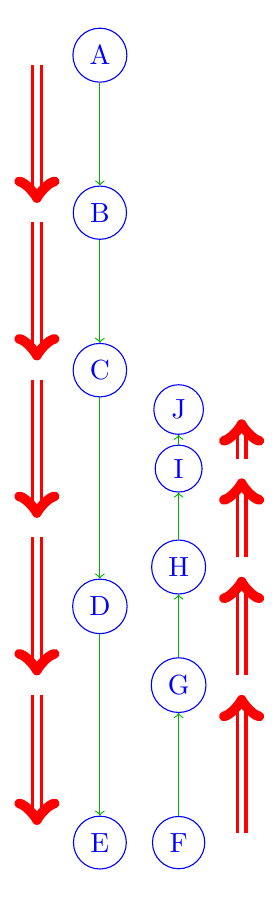
\begin{tikzpicture}[point/.style={circle,draw=blue,text=blue}, vel/.style={draw=green!70!black}, acc/.style={draw=red,very thick, double distance=2pt}]
    
        \node[point] (A) at (0,10) {A};
        \node[point] (B) at (0, 8) {B};
        \node[point] (C) at (0, 6) {C};
        \node[point] (D) at (0, 3) {D};
        \node[point] (E) at (0, 0) {E};
        % upwards accel
        \node[point] (F) at (1, 0) {F};
        \node[point] (G) at (1, 2) {G};
        \node[point] (H) at (1, 3.5) {H};
        \node[point] (I) at (1, 4.75) {I};
        \node[point] (J) at (1, 5.5) {J};
        
        \node (Acc1) at (-0.8, 10) {};
        \node (Acc2) at (-0.8, 8) {};
        \node (Acc3) at (-0.8, 6) {};
        \node (Acc4) at (-0.8, 4) {};
        \node (Acc5) at (-0.8, 2) {};
        \node (Acc11) at (-0.8, .1) {};
        
        \node (Acc6) at (1.8, 0) {};
        \node (Acc7) at (1.8, 2) {};
        \node (Acc8) at (1.8, 3.5) {};
        \node (Acc9) at (1.8, 4.75) {};
        \node (Acc10) at (1.8, 5.5) {};
    	
    	
        \draw[vel, <-] (E) -- (D);
        \draw[vel, <-] (D) -- (C);
        \draw[vel, <-] (C) -- (B);
        \draw[vel, <-] (B) -- (A);
        \draw[vel, ->] (F) -- (G);
        \draw[vel, ->] (G) -- (H);
        \draw[vel, ->] (H) -- (I);
        \draw[vel, ->] (I) -- (J);
        
        \draw[acc, ->] (Acc1) -- (Acc2); 
        \draw[acc, ->] (Acc2) -- (Acc3); 
        \draw[acc, ->] (Acc3) -- (Acc4); 
        \draw[acc, ->] (Acc4) -- (Acc5); 
        \draw[acc, ->] (Acc5) -- (Acc11); 
        
        \draw[acc, ->] (Acc6) -- (Acc7); 
        \draw[acc, ->] (Acc7) -- (Acc8); 
        \draw[acc, ->] (Acc8) -- (Acc9); 
        \draw[acc, ->] (Acc9) -- (Acc10);
    \end{tikzpicture}
    
\end{center}

If there is no change in velocity, there is no acceleration vector. In this case, the would be no red arrow vectors. 
    
Here is another motion diagram, representing an object moving forwards with constant velocity.
\begin{center}
        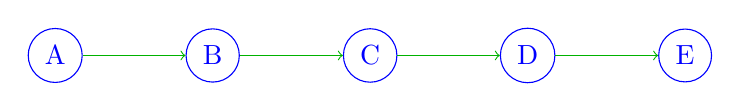
\begin{tikzpicture}[point/.style={circle,draw=blue,text=blue}, vel/.style={draw=green!70!black}, acc/.style={draw=red,very thick, double distance=2pt}]
        
            \node[point] (A) at (2, 0) {A};
            \node[point] (B) at (4, 0) {B};
            \node[point] (C) at (6, 0) {C};
            \node[point] (D) at (8, 0) {D};
            \node[point] (E) at (10, 0) {E};
    
            \draw[vel, ->] (A) -- (B);
            \draw[vel, ->] (B) -- (C);
            \draw[vel, ->] (C) -- (D);
            \draw[vel, ->] (D) -- (E);
        \end{tikzpicture}
\end{center}

% FIXME in-book exercises